\documentclass[12pt]{article}

\usepackage{amsfonts,amssymb}
\usepackage[utf8]{inputenc}
\usepackage[russian]{babel}
\usepackage{amsmath}
\usepackage{amsfonts}
\usepackage[ruled, lined]{algorithm2e}
\usepackage{verbatim}
\usepackage{graphicx}

\textheight=220mm
\textwidth=160mm

\newcommand{\sgn}{\operatorname{sgn}}
\newcommand{\argmax}{\operatorname{argmax}}
\newcommand{\NA}{\operatorname{NA}}
\newcommand{\OR}{\operatorname{ or }}
\newcommand{\LCS}{\operatorname{LCS}}
%\DeclareMathOperator{\sgn}{sgn}

\DeclareGraphicsExtensions{.png}

\title{\bf Лабораторная работа № 2. \\ <<Машинное
Обучение.>>}
\author{А.Е. Оразаев}
\date{}
\begin{document}

\voffset=-20mm
\hoffset=-12mm
\font\Got=eufm10 scaled\magstep2 \font\Got=eufm10

\maketitle

\section{Непараметрическое восстановление плотности.}

\paragraph{1. Добавить команды для загрузки пакетов mvtnorm и np.}
\begin{verbatim}
library('mvtnorm')
library('np')
\end{verbatim}

\paragraph{2. Установите значение размерности данных.}
\begin{verbatim}
dimension = 1
\end{verbatim}
Далее в ходе работы размерность менялась для достижения нужных результатов.

\paragraph{3. Сгенерируйте тестовое множество точек из нормального распределения.}
\begin{verbatim}
MEAN = numeric(dimension)
SIGMA = diag(dimension)
eval_data = rmvnorm(eval_points_number, mean=MEAN, sigma=SIGMA)
\end{verbatim}
Визуализированные данные для размерностей 1, 2 и 3.

\begin{center}
    \fbox{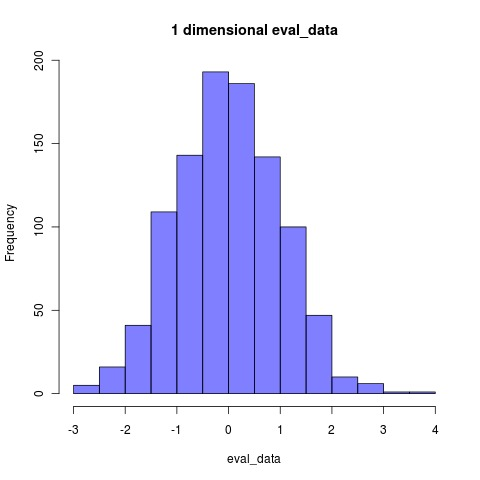
\includegraphics[width=200bp]{imgs/eval_data_dim_1}}
    \fbox{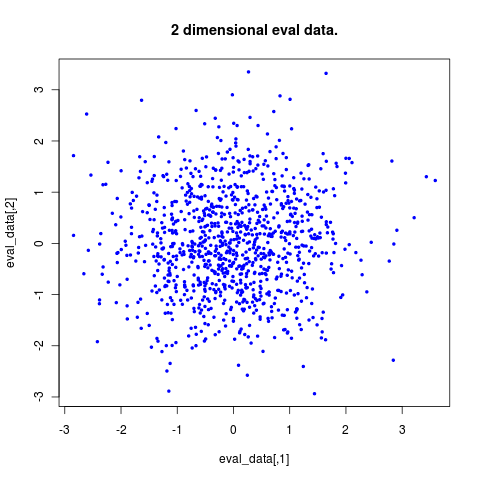
\includegraphics[width=200bp]{imgs/eval_data_dim_2}}
    \fbox{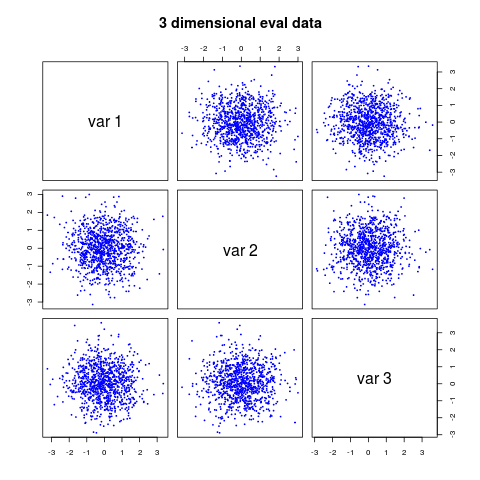
\includegraphics[width=300bp]{imgs/eval_data_dim_3}}
\end{center}

\paragraph{4. Сгенерируйте обучающую выборку из точек из нормального распределения.}
\begin{verbatim}
train_data = rmvnorm(train_points_number, mean=MEAN, sigma=SIGMA)
\end{verbatim}

\paragraph{5. Обучите восстановитель плотности.}
\begin{verbatim}
BWS = numeric(dimension) + 0.5;
density_estimator = npudens(bws=BWS, train_data)
\end{verbatim}

\paragraph{6. Вычислите истинные значения плотности в тестовых точках.}
\begin{verbatim}
groundtruth_values = dmvnorm(eval_data, mean=MEAN, sigma=SIGMA)
\end{verbatim}

\paragraph{7. Вычислите среднюю относительную квадратичную ошибку.}
\begin{verbatim}
mean_relative_square_error = mean(
        ((groundtruth_values - predicted_values) ^ 2) / (groundtruth_values ^ 2))
\end{verbatim}

\paragraph{Полученные графики зависимости величины ошибки от размера обучающей выборки.}
\begin{center}
    \fbox{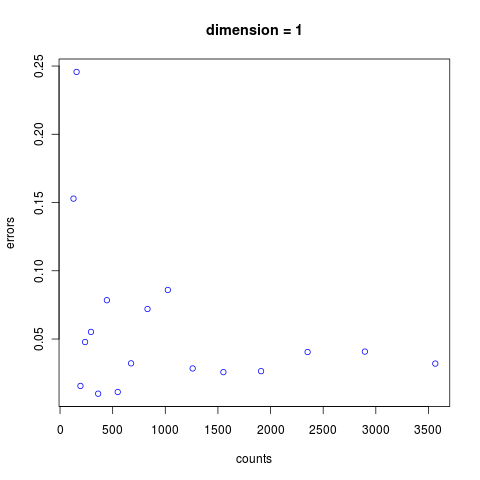
\includegraphics[width=200bp]{imgs/dimension_eq_1}}
    \fbox{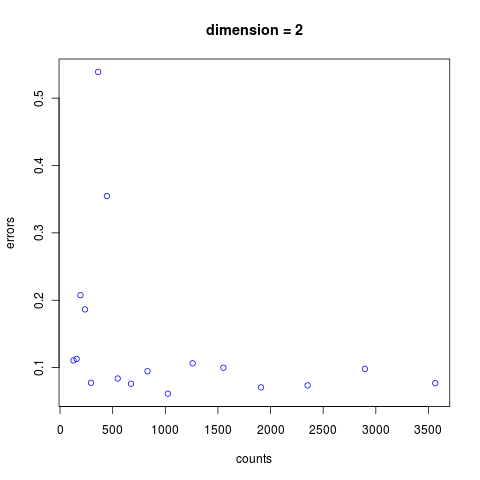
\includegraphics[width=200bp]{imgs/dimension_eq_2}}
    \fbox{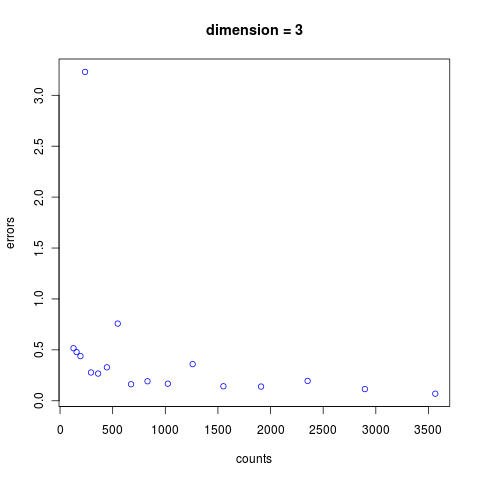
\includegraphics[width=200bp]{imgs/dimension_eq_3}}
\end{center}

\paragraph{Поиск минимального размера обучающей выборки с низкой ошибкой.}
Были поставлены условия достичь ошибки восстановления $ \le 0.05 $. Для
нахождения минимального размера была написана следующая функция:

\begin{verbatim}
getMinimalTrainingDataSizeToBeatErrorThreshold = function(threashold=0.05) {
    trainingDataSize = 1
    meanError = getDensityEstimationError(trainingDataSize)
    while (meanError > threashold) {
        print(sprintf("Size: %d, Error: %f", trainingDataSize, meanError))
        trainingDataSize = trainingDataSize + 1
        meanError = getDensityEstimationError(trainingDataSize)
    }
    print(sprintf("Size: %d, Error: %f", trainingDataSize, meanError))

    return(trainingDataSize)
}
\end{verbatim}

Результаты:
\begin{itemize}
    \item Для размерности 1, размер обучающей выборки 14.
    \item Для размерности 2, размер обучающей выборки 119.
    \item Для размерности 3, размер обучающей выборки >2000
          (Моего терпения не хватило, чтобы дождаться завершения работы скрипта).
\end{itemize}

\end{document}
